\documentclass[10pt,aspectratio=169,american]{beamer}

\usepackage{unicode-math}
\defaultfontfeatures{Scale=MatchLowercase}
\defaultfontfeatures[\rmfamily]{Ligatures=TeX,Scale=1}
\usepackage{lmodern}
\usetheme{metropolis}
\usepackage{microtype}
\UseMicrotypeSet[protrusion]{basicmath}
\usepackage{parskip}
\usepackage{babel}
\usepackage{bookmark}
\usepackage{xurl}
\usepackage{qrcode}
\usepackage{listings}
\usepackage{lstlinebgrd}
% Match the paper's Inconsolata code font without changing the deck's body font.
\newfontfamily\paperCodeFont[Scale=1,BoldFont=Inconsolatazi4-Bold.otf]{Inconsolatazi4-Regular.otf}
\newsavebox{\programInvariantListing}
\newsavebox{\velvetIntroListing}

\definecolor{codeKeyword}{HTML}{204A87}
\definecolor{codeString}{HTML}{4E9A06}
\definecolor{codeOperator}{HTML}{CE5C00}
\definecolor{codeNumber}{HTML}{0000CF}
\definecolor{codeComment}{HTML}{8F5902}
\lstdefinestyle{paperLean}{
  basicstyle=\paperCodeFont\mdseries\color{black}\linespread{1}\fontsize{8.4}{9}\selectfont,
  columns=fullflexible,keepspaces=true,showstringspaces=false,
  frame=none,backgroundcolor=\color{white},
  aboveskip=0pt,belowskip=0pt,mathescape=true,
  alsoletter={_},
  morekeywords={def,method,return,require,ensures,do,let,mut,if,then,else,while,invariant,decreasing,fun,guard,by,prove_correct,loom_solve},
  keywordstyle=\color{codeKeyword}\bfseries,
  identifierstyle=\color{black}\mdseries,
  morestring={[b]"},stringstyle=\color{codeString}\mdseries,
  morecomment={[l]{--}},commentstyle=\color{codeComment}\mdseries\upshape,
  literate={:=}{{\textcolor{codeOperator}{:=}}}2
           {=>}{{\textcolor{codeOperator}{=>}}}2
           {:}{{\textcolor{codeOperator}{:}}}1
           {(}{{\textcolor{codeOperator}{(}}}1
           {)}{{\textcolor{codeOperator}{)}}}1
           {0}{{\textcolor{codeNumber}{0}}}1
           {1}{{\textcolor{codeNumber}{1}}}1
           {2}{{\textcolor{codeNumber}{2}}}1
           {3}{{\textcolor{codeNumber}{3}}}1
           {4}{{\textcolor{codeNumber}{4}}}1
           {5}{{\textcolor{codeNumber}{5}}}1
           {6}{{\textcolor{codeNumber}{6}}}1
           {7}{{\textcolor{codeNumber}{7}}}1
           {8}{{\textcolor{codeNumber}{8}}}1
           {9}{{\textcolor{codeNumber}{9}}}1
}

\urlstyle{same}
\setlength{\emergencystretch}{3em}

\usetikzlibrary{arrows,fit,backgrounds,calc,shapes.symbols}
% Small adjustments to the Metropolis theme used in ../par_incr_presentation.
\metroset{numbering=fraction,progressbar=frametitle}
\setbeamertemplate{navigation symbols}{}
\setbeamercolor{background canvas}{bg=white}

\newcommand{\AIImageCreditFrame}{-1}
\newcommand{\aiimagefooter}{%
  \xdef\AIImageCreditFrame{\number\value{framenumber}}%
}
\setbeamertemplate{frame footer}{%
  \ifnum\value{framenumber}=\AIImageCreditFrame\relax
    {\color{gray}Images are AI-generated}%
  \fi
}

% Eight authors and three affiliations need a more compact cover.
\setbeamerfont{title}{size=\Large}
\setbeamerfont{author}{size=\small,series=\bfseries}
\setbeamerfont{institute}{size=\scriptsize}
\setbeamerfont{date}{size=\small}

% Portraits from https://verse-lab.org/, in paper author order.
\newcommand{\titleAuthor}[3]{%
  \begin{minipage}[t]{0.118\textwidth}
    \centering
    \includegraphics[width=12.5mm,height=12.5mm,keepaspectratio]{assets/authors/#1}\par
    \vspace{1mm}
    {\bfseries\fontsize{6.5}{7.5}\selectfont #2\\#3\par}
  \end{minipage}%
}

% The stock title page's fixed spacing is too tall for this author list at 16:9.
\setbeamertemplate{title page}{%
  \setlength{\parskip}{0pt}
  \vspace*{2mm}
  
\includegraphics[height=9mm]{assets/nus-logo.png}%
  \hspace{8mm}%
  
\includegraphics[height=9mm]{assets/neapolis-logo.png}%
  \hspace{8mm}%
  \raisebox{1mm}{
\includegraphics[height=7mm]{assets/eth-logo.png}}\par
  \vspace{4mm}
  {\usebeamerfont{title}\usebeamercolor[fg]{title}\inserttitle\par}
  \vspace{2mm}
  \usebeamertemplate*{title separator}
  \vspace{3mm}
  \noindent
  \titleAuthor{yueyang.jpg}{Yueyang}{Feng\textsuperscript{1,*}}\hfill
  \titleAuthor{dipesh.jpg}{\underline{Dipesh}}{\underline{Kafle}\textsuperscript{1,*}}\hfill
  \titleAuthor{vladimir.png}{Vladimir}{Gladshtein\textsuperscript{1}}\hfill
  \titleAuthor{vitaly.jpg}{Vitaly}{Kurin\textsuperscript{2}}\hfill
  \titleAuthor{george.jpg}{George}{Pîrlea\textsuperscript{1}}\hfill
  \titleAuthor{qiyuan.jpg}{Qiyuan}{Zhao\textsuperscript{1}}\hfill
  \titleAuthor{peter.jpeg}{Peter}{Müller\textsuperscript{3}}\hfill
  \titleAuthor{ilya.jpg}{Ilya}{Sergey\textsuperscript{1}}\par
  \vspace{4mm}
  {\usebeamerfont{institute}\insertinstitute\par}
  \vspace{3mm}
  {\usebeamerfont{date}\insertdate\par}
}

\pdfstringdefDisableCommands{%
  \def\textsuperscript#1{}%
  \def\underline#1{#1}%
  \def\\{ }%
}

% Keep the PDF metadata readable (without affiliation markers or TeX).
\hypersetup{
  pdftitle={Certified program synthesis with a multi-modal verifier},
  pdfauthor={Yueyang Feng, Dipesh Kafle, Vladimir Gladshtein, Vitaly Kurin, George Pîrlea, Qiyuan Zhao, Peter Müller, Ilya Sergey}
}


% Compact diagrams shared by the three invariant-validation slides.
\newcommand{\invariantFlow}[3]{%
\begin{center}
\begin{tikzpicture}[
  stage/.style={draw=teal!65,fill=teal!4,rounded corners=2pt,
    minimum width=36mm,minimum height=10mm,align=center,font=\small},
  flow/.style={->,thick,draw=mLightBrown}]
\node[stage] (a) at (0,0) {#1};
\node[stage] (b) at (4.7,0) {#2};
\node[stage] (c) at (9.4,0) {#3};
\draw[flow] (a) -- (b);
\draw[flow] (b) -- (c);
\end{tikzpicture}
\end{center}%
}
\lstdefinestyle{reviewJSON}{
  basicstyle=\paperCodeFont\mdseries\color{black}\linespread{1}\fontsize{7.7}{8.3}\selectfont,
  columns=fullflexible,keepspaces=true,showstringspaces=false,
  aboveskip=0pt,belowskip=0pt,mathescape=true,
  morestring={[b]"},stringstyle=\color{codeKeyword}\mdseries,
  morekeywords={false,true},keywordstyle=\color{codeOperator}\bfseries
}
\hypersetup{
  pdflang={en-US},
  colorlinks=true,
  linkcolor=teal,
  urlcolor=teal,
  pdfcreator={XeLaTeX / Beamer}
}

\title{Certified program synthesis\\
with a multi-modal verifier}
\author{Yueyang Feng\textsuperscript{1,*}, \underline{Dipesh Kafle}\textsuperscript{1,*},
Vladimir Gladshtein\textsuperscript{1}, Vitaly Kurin\textsuperscript{2}\\
George Pîrlea\textsuperscript{1}, Qiyuan Zhao\textsuperscript{1},
Peter Müller\textsuperscript{3}, Ilya Sergey\textsuperscript{1}}
\institute{\textsuperscript{1}National University of Singapore\quad
\textsuperscript{2}Neapolis University Pafos\quad
\textsuperscript{3}ETH Zurich\\[0.4em]
\textsuperscript{*}Joint first authors}
\date{ASE ’26 · October 15, 2026 · Munich, Germany}

\begin{document}

\begin{frame}
\titlepage
\end{frame}

\begin{frame}{Motivation}
\aiimagefooter
\centering
{\large AI writes code for us. An idea becomes an implementation in seconds.\par}
\vspace{1mm}
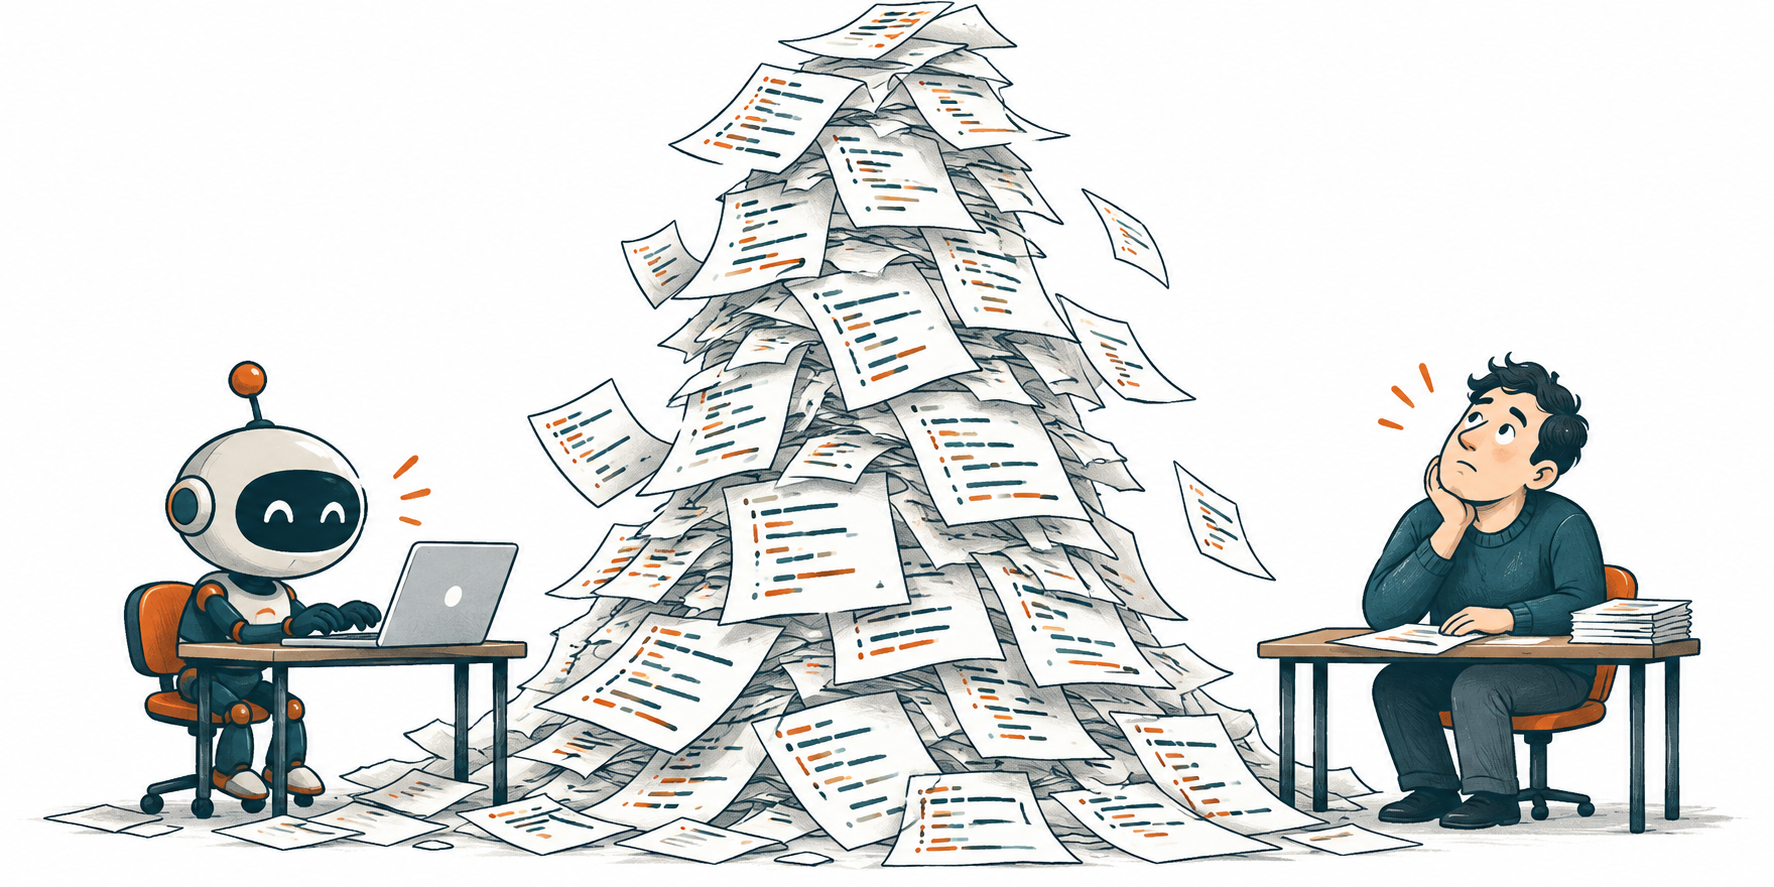
\includegraphics[width=0.86\textwidth,height=36mm,keepaspectratio]{assets/ai-code-review.png}

\pause

{\Large\bfseries\color{mLightBrown}Who reviews all this code?\par}
\vspace{1mm}
{\small Generating code is fast. Establishing confidence still takes tremendous amount of work.\par}

\end{frame}

\begin{frame}{Motivation}
\aiimagefooter
\begin{columns}[c,onlytextwidth]
\begin{column}{0.57\textwidth}
\centering

\includegraphics[width=\linewidth,height=33mm,keepaspectratio]{assets/ai-proof-checking.png}

{\large Ask the AI for a proof, too.\par}
\end{column}
\begin{column}{0.39\textwidth}
\small
\textbf{Fermat's Last Theorem}\\
13 million lines of Lean;\\
machine-checked proof.\\[-0.5mm]
{\scriptsize\href{https://www.anthropic.com/news/formalizing-fermats-last-theorem}{Anthropic, September 2026}}

\vspace{3mm}
\textbf{Navier--Stokes}\\
Proof released with a\\
Lean formalization.\\[-0.5mm]
{\scriptsize\href{https://openai.com/index/navier-stokes-solution/}{OpenAI, September 2026}}
\end{column}
\end{columns}

\vspace{4mm}
\centering
\uncover<2->{%
\textbf{In an ideal world:}\\[1mm]
User gives a task description;\\
AI gives a specification + implementation + proof.
}

\end{frame}

\begin{frame}{Our goal: Certified synthesis from natural language}
\setlength{\parskip}{0pt}
Generate a runnable program and a checked correctness proof from an English task.

\vspace{10mm}
\uncover<2->{{\centering\textbf{Two key challenges}\par}}
\vspace{4mm}
\begin{columns}[T,onlytextwidth]
\begin{column}{0.47\textwidth}
\uncover<2->{%
\textbf{\color{teal}Assessing specifications effectively}\par
\vspace{3mm}
Does the specification capture\\
the intended task?\par
}
\end{column}
\begin{column}{0.47\textwidth}
\uncover<3->{%
\textbf{\color{teal}Constructing proofs efficiently}\par
\vspace{3mm}
Can we complete the proof\\
within a limited budget?\par
}
\end{column}
\end{columns}

\end{frame}

\begin{frame}{Outline}
\centering
\begin{tikzpicture}[
  stop/.style={circle,draw=teal,fill=teal!5,line width=1pt,
    minimum size=12mm,inner sep=0pt,font=\Large\bfseries,text=teal},
  heading/.style={font=\large\bfseries,text=mDarkTeal,align=center},
  detail/.style={font=\small,align=center,text width=38mm},
  journey/.style={->,line width=1pt,draw=mLightBrown}]
\path[use as bounding box] (-2,-3.4) rectangle (11.4,0.7);
\node[stop] at (0,0) {1};
\node[heading] at (0,-1.25) {The idea};
\node[detail,anchor=north] at (0,-1.85) {Multi-modal\\verification};
\uncover<2->{%
  \draw[journey] (0.85,0) -- (3.85,0);
  \node[stop] at (4.7,0) {2};
  \node[heading] at (4.7,-1.25) {The pipeline};
  \node[detail,anchor=north] at (4.7,-1.85) {Inside LeetProof};
}
\uncover<3->{%
  \draw[journey] (5.55,0) -- (8.55,0);
  \node[stop] at (9.4,0) {3};
  \node[heading] at (9.4,-1.25) {The evidence};
  \node[detail,anchor=north] at (9.4,-1.85) {What the results show};
}
\end{tikzpicture}
\end{frame}

\begin{frame}{Our approach: Multi-modal verification}
\begin{uncoverenv}<2->
\begin{columns}[T,onlytextwidth]
\begin{column}{0.30\textwidth}
\textbf{\color{teal}Test}

Check examples with unit tests; search for counterexamples with PBT.
\end{column}
\begin{column}{0.30\textwidth}
\textbf{\color{teal}Automate}

Discharge goals with SMT and Lean automation like \texttt{grind}.
\end{column}
\begin{column}{0.30\textwidth}
\textbf{\color{teal}Prove interactively}

Complete proofs when automation gets stuck.
\end{column}
\end{columns}
\end{uncoverenv}

\vspace{8mm}
\uncover<3->{\href{https://velvetprover.dev/}{\textbf{Velvet}} combines these \textbf{\textit{modes}} for imperative programs in Lean.\par}

\vspace{5mm}
\uncover<4->{We present \textbf{\color{mLightBrown}LeetProof}, which uses multi-modality to turn English tasks into verified programs.\par}

\end{frame}

\begin{frame}[fragile]{Velvet 101}
\setlength{\parskip}{0pt}
\begin{lrbox}{\velvetIntroListing}
\begin{minipage}{0.70\textwidth}
\begin{lstlisting}[
  style=paperLean,
  linebackgroundcolor={\color{white}\ifnum\value{lstnumber}=2 \color{blue!9}\fi\ifnum\value{lstnumber}>7 \ifnum\value{lstnumber}<10 \color{yellow!16}\fi\fi\ifnum\value{lstnumber}>14 \color{green!12}\fi},
  linebackgroundheight=6.8pt,linebackgrounddepth=2.2pt
]
method IsNonPrime (n : Nat) return (result : Bool)
  ensures result = true $\leftrightarrow$ $\neg$isPrime n
  do
    if n $\leq$ 1 then return true
    let mut i : Nat := 2
    let mut ret : Bool := false
    while i * i $\leq$ n
    invariant $\neg$ret $\leftrightarrow$ $\forall$d, 2 $\leq$ d $\land$ d < i $\to$ n % d $\neq$ 0
    invariant i $\geq$ 2 $\land$ (i - 1) * (i - 1) $\leq$ n
    do
      if n % i = 0 then ret := true
      i := i + 1
    return ret

prove_correct IsNonPrime by
  loom_solve  -- automated VC discharge
  ...         -- remaining interactive proof
\end{lstlisting}
\end{minipage}
\end{lrbox}
\begin{tikzpicture}
\node[inner sep=0pt,anchor=west] (velvetCode) at (0,0)
  {\usebox{\velvetIntroListing}};
\uncover<2->{%
\begin{scope}[overlay,
  introCallout/.style={cloud,cloud puffs=10,cloud puff arc=110,
    aspect=2,thick,text width=18mm,align=center,inner sep=0.5mm,
    font=\fontsize{8}{9}\selectfont}]
\coordinate (contractRow) at
  ($(velvetCode.north east)!0.09!(velvetCode.south east)$);
\coordinate (loopRow) at
  ($(velvetCode.north east)!0.47!(velvetCode.south east)$);
\coordinate (proofRow) at
  ($(velvetCode.north east)!0.91!(velvetCode.south east)$);
\node[introCallout,draw=codeKeyword,fill=blue!6] (contractNote)
  at ($(contractRow)+(22mm,-4mm)$) {Postcondition};
\node[introCallout,draw=mLightBrown,fill=yellow!12] (loopNote)
  at ($(loopRow)+(22mm,0)$) {Loop invariants};
\node[introCallout,draw=teal,fill=green!8] (proofNote)
  at ($(proofRow)+(22mm,0)$) {Automation\newline + interactive\newline proofs};
\draw[->,thick,codeKeyword] (contractNote.west) -- ([xshift=-3mm]contractRow);
\draw[->,thick,mLightBrown] (loopNote.west) -- ([xshift=-3mm]loopRow);
\draw[->,thick,teal] (proofNote.west) -- ([xshift=-3mm]proofRow);
\end{scope}%
}
\end{tikzpicture}\par

\end{frame}

\begin{frame}{LeetProof pipeline}
LeetProof orchestrates the entire pipeline from natural language to a verified implementation in the following phases:

\vspace{6mm}
\begin{columns}[T,onlytextwidth]
\begin{column}{0.28\textwidth}
{\large\textbf{1. Generate\\specification}\par}
\small
\alert<2->{Capture the intent} of an English description in a Lean specification.
\end{column}
\begin{column}{0.05\textwidth}
\vspace{10mm}
{\large\color{mLightBrown}$\longrightarrow$}
\end{column}
\begin{column}{0.28\textwidth}
{\large\textbf{2. Synthesize\\program}\par}
\small
\textbf{Plain Lean:} Generate a functional implementation.

\vspace{2mm}
\textbf{Velvet:} Generate an imperative implementation, then \alert<2->{infer and annotate loops with invariants}.
\end{column}
\begin{column}{0.05\textwidth}
\vspace{10mm}
{\large\color{mLightBrown}$\longrightarrow$}
\end{column}
\begin{column}{0.28\textwidth}
{\large\textbf{3. Verify the\\program}\par}
\small
Prove that the synthesized program satisfies the specification.
\end{column}
\end{columns}

\end{frame}

\begin{frame}{Specification generation}
\begin{itemize}
\setlength{\itemsep}{6mm}
\item<1-> \textbf{Capturing intent is difficult} for LLMs, and even humans.
\item<2-> Intent capture cannot be guaranteed, but we can effectively \textbf{\color{mLightBrown}search for mismatches}.
\end{itemize}

\end{frame}

\begin{frame}{Specification generation}
\begingroup
\large\textbf{Step 1: Check the LLM's understanding}\par
\endgroup
\vspace{4mm}

\begin{columns}[c,onlytextwidth]
\begin{column}{0.28\textwidth}
\centering\textbf{Task description}
\end{column}
\begin{column}{0.08\textwidth}
\centering{\Large\color{mLightBrown}$\longrightarrow$}
\end{column}
\begin{column}{0.58\textwidth}
\textbf{Formal specification + example inputs and outputs}
\end{column}
\end{columns}

\vspace{5mm}
Reuse examples from the problem statement and ask the LLM for more\\
based on its interpretation (about ten in total).

\vspace{3mm}
\begin{center}
\begin{tabular}{@{}l@{\hspace{15mm}}l@{}}
\textbf{Input} & \textbf{Expected output}\\[1mm]
\texttt{[4, 1, 2, 3]} & \texttt{true}\\
\texttt{[2, 1, 3, 4]} & \texttt{false}\\
\texttt{[1, 1, 1]} & \texttt{true}
\end{tabular}
\end{center}

\end{frame}

\begin{frame}{Specification generation}
\setlength{\parskip}{0pt}
\begingroup
\large\textbf{Step 2: Gaining confidence in the generated specification}\par
\endgroup
\vspace{3mm}

\uncover<2->{We can prove that the examples satisfy the precond and postcond. But, proving each example can be expensive.}\\
\uncover<3->{\textbf{Key insight: Search for counterexamples with property-based testing (PBT).}}

\vspace{4mm}
\begin{tabular}{@{}p{0.26\textwidth}@{\hspace{4mm}}p{0.66\textwidth}@{}}
\uncover<4->{\textbf{\color{teal}Input validity}} & \uncover<4->{Does the input satisfy the precondition?}\\[4mm]
\uncover<5->{\textbf{\color{teal}Expected output}} & \uncover<5->{Does the intended answer satisfy the postcondition?}\\[4mm]
\uncover<6->{\textbf{\color{teal}Output uniqueness}} & \uncover<6->{Does the specification also admit a different answer?}
\end{tabular}

\vspace{5mm}
\uncover<6->{Keep the input fixed; sample alternative outputs by mutating the expected output.}

\end{frame}

\begin{frame}[fragile]{Specification generation}
\setlength{\parskip}{0pt}
{\small Task: Return whether the array is sorted and rotated.\par}
\vspace{4mm}

\begin{overlayarea}{\textwidth}{21mm}
\begin{onlyenv}<1-2>
{\large\textbf{Candidate specification 1}\par}
\vspace{3mm}
\begin{lstlisting}[style=paperLean,basicstyle=\paperCodeFont\mdseries\color{black}\fontsize{10}{12}\selectfont]
def postcondition (nums : Array Int) (result : Bool) :=
  result = true $\textcolor{red!75!black}{\to}$ rotSortedProp nums
\end{lstlisting}
\end{onlyenv}
\begin{onlyenv}<3>
{\large\textbf{Candidate specification 2}\par}
\vspace{3mm}
\begin{lstlisting}[style=paperLean,basicstyle=\paperCodeFont\mdseries\color{black}\fontsize{10}{12}\selectfont]
def postcondition (nums : Array Int) (result : Bool) :=
  result = true $\textcolor{teal}{\leftrightarrow}$ rotSortedProp nums
\end{lstlisting}
\end{onlyenv}
\end{overlayarea}

\begin{overlayarea}{\textwidth}{29mm}
\only<2>{%
With $\to$, always returning \texttt{false} satisfies the specification.\par
\vspace{4mm}
\textbf{Output uniqueness test}\par
\texttt{[1, 2, 3]}:\quad \texttt{true} $\longrightarrow$ \texttt{false}\quad postcondition still holds!\par
}
\end{overlayarea}

\begin{overlayarea}{\textwidth}{9mm}
\centering
\only<2>{{\Large\bfseries\color{red!75!black}Rejected by PBT\par}}
\only<3>{{\Large\bfseries\color{teal}Approved by pipeline\par}}
\end{overlayarea}
\end{frame}

\begin{frame}[fragile]{Invariant inference}
\setlength{\parskip}{0pt}
{\large\textbf{Step 1: Generate candidate invariants}\par}
\vspace{5mm}
\begin{columns}[T,onlytextwidth]
\begin{column}{0.28\textwidth}
\textbf{\color{teal}Program}\par
\vspace{4mm}
\begin{lstlisting}[style=paperLean,basicstyle=\paperCodeFont\mdseries\color{black}\fontsize{10}{11}\selectfont]
while i < n
do
  ...
\end{lstlisting}
\end{column}
\begin{column}{0.19\textwidth}
\uncover<2->{%
\centering
{\small LLM proposes\\annotations\par}
\vspace{2mm}
{\Huge\color{mLightBrown}$\longrightarrow$\par}
}
\end{column}
\begin{column}{0.53\textwidth}
\begin{uncoverenv}<2->
\textbf{\color{teal}Annotated program}\par
\vspace{4mm}
\begin{lstlisting}[
  style=paperLean,
  basicstyle=\paperCodeFont\mdseries\color{black}\fontsize{9.5}{11}\selectfont,
  numbers=none,
  linebackgroundcolor={\color{white}\ifnum\value{lstnumber}>1 \ifnum\value{lstnumber}<5 \color{yellow!16}\fi\fi}
]
while i < n
  invariant "inv_bounds" (i $\leq$ n)
  invariant "inv_drops_count" (...)
  decreasing n - i
do
  ...
\end{lstlisting}
\end{uncoverenv}
\end{column}
\end{columns}

\end{frame}

\begin{frame}[fragile]{Invariant inference}
\setlength{\parskip}{0pt}
{\large\textbf{Step 2: Validate invariants (automation)}\par}
\vspace{3mm}
\textbf{Discharge obligations automatically using SMT / Lean's automation.}
\vspace{3mm}

\vspace{3mm}
{\small\color{teal}A simplified obligation for illustrative purpose\par}
\vspace{2mm}
\begin{lstlisting}[style=paperLean,basicstyle=\paperCodeFont\mdseries\color{black}\fontsize{10}{11}\selectfont]
i n : Nat
h : i < n
$\vdash$ i + 1 $\leq$ n $\land$ n - (i + 1) < n - i
\end{lstlisting}

\vspace{5mm}
\uncover<2->{%
For the final program of our running example, 14/18 VCs were discharged using automation.\par
}
\end{frame}

\begin{frame}[fragile]{Invariant inference}
\setlength{\parskip}{0pt}
{\large\textbf{Step 2: Validate invariants (counterexample search)}\par}
\vspace{3mm}

\vspace{3mm}
{\small\color{teal}A candidate invariant, with $=$ changed to $<$.\par}
\vspace{2mm}
\begin{lstlisting}[
  style=paperLean,escapeinside={|}{|},backgroundcolor=\color{yellow!16}
]
invariant "inv_drops_count" (drops |\colorbox{red!20}{\paperCodeFont =}\,\colorbox{green!20}{\paperCodeFont <}| (Finset.filter
  (fun k : Nat => nums[(k + 1) % n]! < nums[k]!)
  (Finset.range i)).card)
\end{lstlisting}

\vspace{5mm}
\begin{uncoverenv}<2->
\begin{lstlisting}[
  basicstyle=\paperCodeFont\mdseries\color{black}\fontsize{8}{9}\selectfont,
  columns=fullflexible,keepspaces=true,showstringspaces=false,
  backgroundcolor=\color{red!7},aboveskip=0pt,belowskip=0pt
]
[velvet_plausible_test] FAIL:
invariant "inv_drops_count" doesn't hold
nums = #[-18, 10, -13, 11, 8, 17, 13, -19, 15, -1, -27, -25]
\end{lstlisting}
\end{uncoverenv}
\end{frame}

\begin{frame}{RQ1: Specification quality}
\setlength{\parskip}{0pt}
\textbf{Generating specifications from English tasks}\par
\vspace{7mm}
\begin{columns}[c,onlytextwidth]
\begin{column}{0.44\textwidth}
\centering
{\color{teal}\bfseries\fontsize{36}{40}\selectfont 97.4\%\par}
\vspace{2mm}
\textbf{Equivalent or defensible\textsuperscript{*}}\par
\end{column}
\begin{column}{0.50\textwidth}
\textbf{188 VERINA problems}\par
\vspace{5mm}
\begin{tabular}{@{}r@{\hspace{3mm}}l@{}}
\textbf{150} & Equivalent to reference\\[3mm]
\textbf{33} & Defensible differences
\end{tabular}\par
\end{column}
\end{columns}

\vspace{12mm}
{\footnotesize\textsuperscript{*}Defensible: justified differences due to reference errors, valid precondition variations, or ambiguous descriptions.\par}
\end{frame}

\begin{frame}{RQ1: Specification quality}
\setlength{\parskip}{0pt}
\textbf{PBT uncovers issues in human-written benchmarks}\par
\vspace{6mm}
\begin{columns}[T,onlytextwidth]
\begin{column}{0.47\textwidth}
\centering
\textbf{VERINA}\par
\vspace{3mm}
\begin{minipage}[c][22mm][c]{\linewidth}
\centering
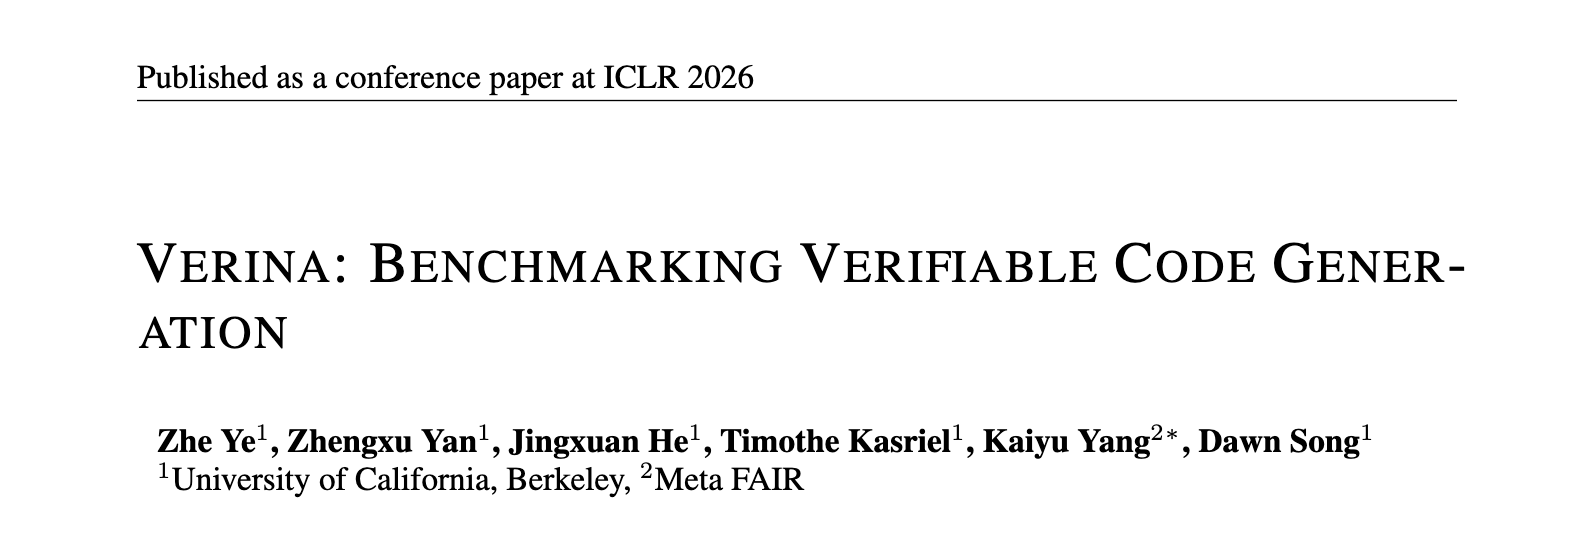
\includegraphics[width=\linewidth,height=22mm,keepaspectratio,trim={30bp 77.5bp 30bp 75bp},clip]{assets/Verina.png}
\end{minipage}\par
\vspace{4mm}
{\Large\bfseries\color{mLightBrown}13 issues}\par
\end{column}
\begin{column}{0.47\textwidth}
\centering
\textbf{CLEVER}\par
\vspace{3mm}
\begin{minipage}[c][22mm][c]{\linewidth}
\centering
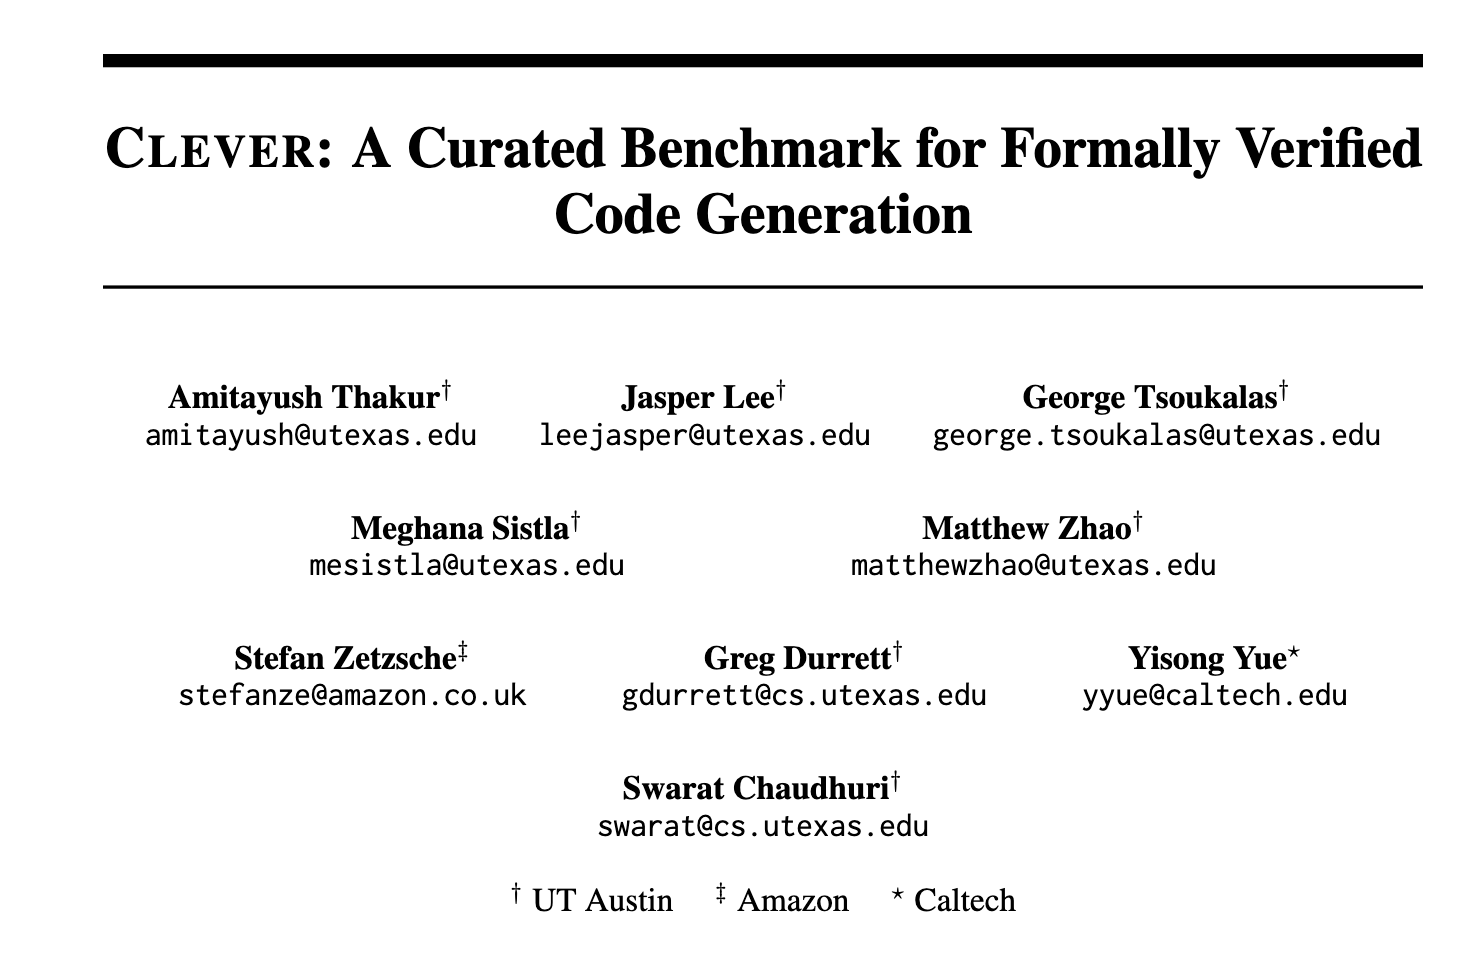
\includegraphics[width=\linewidth,height=22mm,keepaspectratio,trim={0bp 317.5bp 0bp 40bp},clip]{assets/Clever.png}
\end{minipage}\par
\vspace{4mm}
{\Large\bfseries\color{mLightBrown}18 issues}\par
\end{column}
\end{columns}
\vspace{6mm}
{\centering Found without LLM assistance.\par}
\end{frame}

\begin{frame}{Evaluation: RQ2 --- Certified synthesis}
\setlength{\parskip}{0pt}
\begingroup
\large\textbf{More certified solutions with Velvet compared to functional Lean, at the same cost}\par
\endgroup
\vspace{4mm}
\textbf{Fully proven (GPT-5.2):} Lean 17/50; Velvet 28/50.
\vspace{3mm}

\centering
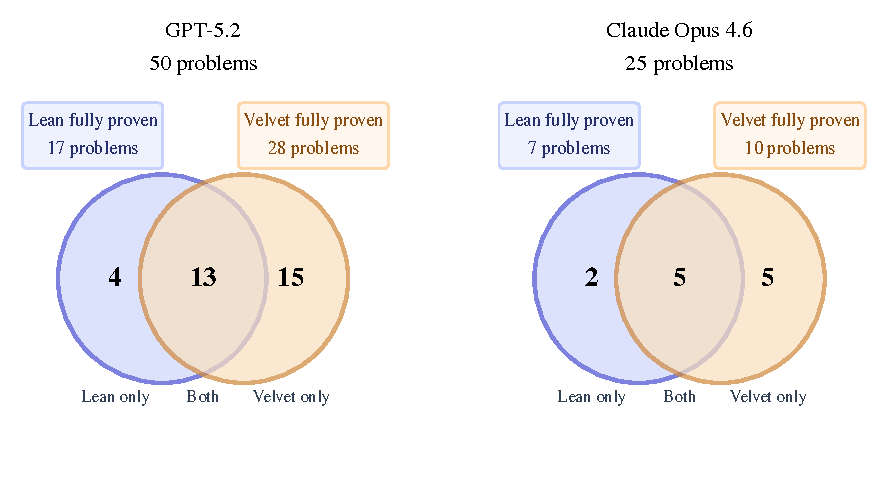
\includegraphics[height=49mm,trim={0bp 35bp 211.827bp 82bp},clip]{assets/backend-overlap-venn.pdf}

\end{frame}

\begin{frame}{Evaluation: RQ3 and RQ4}
\setlength{\parskip}{0pt}
\begin{columns}[T,onlytextwidth]
\begin{column}{0.46\textwidth}
{\large\textbf{\color{teal}RQ3: Closing the remaining proofs}}\par
\vspace{3mm}
Can additional proof effort close the remaining goals?\par
\vspace{4mm}
{\small Partially proven programs completed by Aristotle:\par}
\vspace{3mm}
\begin{tabular}{@{}l@{\hspace{8mm}}r@{}}
Lean & \textbf{23 / 30}\\[3mm]
Velvet & \textbf{\color{teal}18 / 18}
\end{tabular}
\end{column}
\begin{column}{0.46\textwidth}
\begin{uncoverenv}<2->
{\large\textbf{\color{teal}RQ4: Across different LLMs}}\par
\vspace{3mm}
Does the advantage hold with another model?\par
\vspace{4mm}
{\small Fully proven programs at \$5 per problem:\par}
\vspace{3mm}
\begin{tabular}{@{}l@{\hspace{4mm}}r@{\hspace{4mm}}r@{}}
 & Lean & Velvet\\[2mm]
GPT-5.2 & 17/50 & \textbf{\color{teal}28/50}\\[3mm]
Opus 4.6 & 7/25\textsuperscript{*} & \textbf{\color{teal}10/25\textsuperscript{*}}
\end{tabular}\par
\vspace{5mm}
{\footnotesize\textsuperscript{*}25 problems chosen at random from the 50 evaluated with GPT-5.2.\par}
\end{uncoverenv}
\end{column}
\end{columns}
\end{frame}

\begin{frame}{Summary}
\setlength{\parskip}{0pt}
\begingroup
\small
\begin{columns}[T,onlytextwidth]
\begin{column}{0.47\textwidth}
\textbf{\color{teal}What have we seen}\par
\vspace{3mm}
\begin{itemize}
\setlength{\itemsep}{1.5mm}
\item<2-> Certified synthesis needs both \textbf{faithful specifications and complete proofs}.
\item<3-> Testing \textbf{rejects bad candidates} before we spend effort proving them.
\item<4-> LeetProof uses Velvet's multiple modes to \textbf{certify more programs within the same budget}.
\end{itemize}
\end{column}
\begin{column}{0.47\textwidth}
\uncover<5->{\textbf{\color{teal}Interesting future directions}}\par
\vspace{3mm}
\begin{itemize}
\setlength{\itemsep}{1.5mm}
\item<5-> \textbf{Certified synthesis of protocols and distributed systems.}
\item<6-> \textbf{Going Beyond functional correctness.}
\end{itemize}
\end{column}
\end{columns}
\endgroup

\vspace{3mm}
\uncover<7->{%
\centering
\begin{tabular}{@{}c@{\hspace{14mm}}c@{\hspace{14mm}}c@{\hspace{14mm}}c@{}}
\qrcode[height=17mm]{https://verse-lab.org/} &
\qrcode[height=17mm]{https://github.com/verse-lab/velvet/} &
\qrcode[height=17mm]{https://zenodo.org/records/22046794} &
\qrcode[height=17mm]{https://verse-lab.org/papers/leetproof-ase26.pdf}\\[1mm]
\small\href{https://verse-lab.org/}{Verse Lab} &
\small\href{https://github.com/verse-lab/velvet/}{Velvet} &
\small\href{https://zenodo.org/records/22046794}{Artifact} &
\small\href{https://verse-lab.org/papers/leetproof-ase26.pdf}{Paper}
\end{tabular}\par
\vspace{2mm}
{\large\textbf{\color{teal}Thank you!}\par}
}

\end{frame}

\end{document}
